\subsection{Penalty-based formalism}

The second approach to solve the triangle-to-triangle  distance problem by parameterisation of the triangles such that the distance between them is formulated as a quadratic function. The approach is an iterative solution and it is approximated with the Newton method.

The method rely on the optimization-based formulation of the distance between two points. Let $x$ and $y$ be two points, belonging respectively to triangle $T_1$ and $T_2$. Assuming that points $A, B, C$ are vertices of $T_1$ and that points $D, E, F$ are vertices of $T_2$, $x$ and $y$ can be defined using the following equations: 
\begin{align*}
T_{1}:x(a,b)=A+(B-A) \cdot a+(C-A)\cdot b
\end{align*}
\begin{align*}
T_{2}:y(g,d)=D+(E-D) \cdot g+(F-D) \cdot d
\end{align*} 
To find the minimum distance between $T_1$ and $T_2$ and the corresponding two closest points $P$, $Q$ on the two triangles we minimize
\begin{align*}
f\left(a,b,c,d\right)=\left\Vert x\left(a,b\right)-y\left(c,d\right)\right\Vert ^{2}
\end{align*} 

What has to be noted is that $x$ and $y$ have to stay within the area of the two triangles. The four parameters of the function $f$ have to comply with six inequality constraints:
\begin{align*}
min_{a,b,g,d} f(a,b,g,d)
\end{align*}  
$$such \:that: \: \{a\geq0,b\geq0, a+b\leq1, d\geq0, g\geq0, g+d\leq1 \}$$ 


\begin{figure}[htb]
  \begin{center}
    \includegraphics[width=0.6\textwidth]{sketches/c.png}
  \end{center}
  \caption{
    Example of minimum distance and the corresponding barycentric points (parameters of objective function) on a pair of triangles in 3D. Triangle X:T1 has points A, B, C where barymetric parameters a,b correspond to point $x$ on the triangle. Triangle Y:T2 has points D,E,F where barymetric parameters g,d correspond to a point $x$. The two defined barymetric points define the minimum distance between the two triangles in 3D.
  }
  \label{figure:barycentric_contact}
\end{figure}

To enforce the constraints the problem is transformed into a series of unconstrained problems with the augmentation of the objective function $f$ using the penalty-based method. The penalty function penalizes the iteration so that the boundaries of the feasible region are valid. Although there are factors that determine the number of iterations required the tuned-to-the-problem parameters yield a good number of Newton iterations that cannot be reduced to less than two; (initial guess to penalized boundary step, correction step).

\begin{figure}[htb]
  \begin{center}
    \includegraphics[width=0.5\textwidth]{sketches/penalty.png}
  \end{center}
  \caption{
Illustration of a 2D problem showing the penalty function (red line) penalizing the objective function (black line) f(x) under a constraint $a$ (dash line) to create the feasible region (blue line).
  }
  \label{figure:penaltyfunction}
\end{figure}

This approach adds a penalty term to the objective function to penalize the solution when outside of the feasible region: 
\begin{equation}\label{eq:penalty}
P(x)=f(x)+r\sum_{i=1...6}max(0,c(x_{i}))^{2}
\end{equation}
Where r is the penalty parameter (Figure \ref{}). Newton iterations always converge to a solution slightly on the outside of the feasible region. Convergence can be controlled by the r parameter that controls the sharpness of the curve for the constraints. One aspect that requires care however is the invertibility of the Hessian $\nabla\nabla P$. 

Furthermore the problem is ill conditioned and a Quasi-Newton method is used. The Hessian matrix is not invertible so it is not possible to solve the direction of the search by computing the Hessian and gradient. This illustrates the fact that $f$ has multiple minima and $\nabla\nabla f$ is singular. Consequently, $\nabla\nabla P$ is also singular inside of the feasible region. The ill conditioning is caused by the problem definition itself, where there is a state where there are multiple solutions to the problem based on the orientation of the two triangles. This is also revealed by the two zero eigenvalues of the Hessian. Because of the ill-conditioning, we use a quasi-Newton approach, where the Hessian is approximated by a perturbed operator $\nabla\nabla P + \epsilon I$. $I$ is an identity matrix and $\epsilon$ is suitably small.

\begin{algorithm}
	\protect\caption{\label{alg4}Penalty Solver.}
	\begin{algorithmic}[1]
	
	\Function{Penalty}{A, B, C, D, E, F, rho, tol}

		\State $BA~=~B-A;~CA~=~C-A;~ED~=~E-D;~FD~=~F-D;$

		\State $hf~=~{[}2{*}BA{*}BA',~2{*}CA{*}BA',-2{*}ED{*}BA',-2{*}FD{*}BA';$

		\State $2{*}BA{*}CA',~2{*}CA{*}CA',-2{*}ED{*}CA',-2{*}FD{*}CA';$

		\State $2{*}BA{*}ED',-2{*}CA{*}ED',~2{*}ED{*}ED',~2{*}FD{*}ED';$

		\State $2{*}BA{*}FD',-2{*}CA{*}FD',~2{*}ED{*}FD',~2{*}FD{*}FD'{]};$

		\State $x~=~{[}0.33;~0.33;~0.33;~0.33{]};$

		\For{i=1:99}

			\State $X~=~A+BA{*}x(1)~+~CA{*}x(2);$

			\State $Y~=~D+ED{*}x(3)~+~FD{*}x(4);$

			\State $gf~=~{[}2{*}(X-Y){*}BA';~2{*}(X-Y){*}CA';~-2{*}(X-Y){*}ED';~-2{*}(X-Y){*}FD'{]};$

			\State $h~=~{[}-x(1);~-x(2);~x(1)+x(2)-1;~-x(3);~-x(4);~x(3)+x(4)-1{]};$

			\State $dh~=~{[}-1,~0,~1,~0,~0,~0;~0,~-1,~1,~0,~0,~0;$

			\State $0,~0,~0,~-1,~0,~1;~0,~0,~0,~0,~-1,~1{]};$

			\State $mask~=~h'~$>$=~0;$

			\State $dmax~=~dh.{*}~{[}mask;~mask;~mask;~mask{]};$

			\State $gra~=~gf~+~rho~{*}~dmax~{*}~max(0,h(:));$

			\State $hes~=~hf~+~rho{*}dmax{*}dmax'~+~eye(4,4)/rho^2;$

			\State $dx~=~hes\textbackslash{}gra;$

			\State $DX~=~BA{*}dx(1)~+~CA{*}dx(2);$

			\State $DY~=~ED{*}dx(3)~+~FD{*}dx(4);$

			\State $error~=~sqrt(DX{*}DX'+DY{*}DY');$

			\If{error~$<$~tol}
				\State $BREAK;$
			\EndIf

			\State $x~=~x~-~dx;$

		\EndFor

	\EndFunction
	\end{algorithmic}

\end{algorithm}


The penalty algorithm as shown in Algorithm \ref{} accepts A, B, C, D, E, F vector coordinates for triangle T1(A, B, C), T2(D, E, F) as well as the required parameters for the algorithm to be solved. Rho is the penalty parameter that controls the steepness of the P(x) function (equation \ref{eq:penalty}) , eps is the perturbation parameter for the hessian matrix of the problem along its diagonal to make the matrix solvable. Tol is the tolerance for convergence (Floating point accuracy). In line 23 of Algorithm \ref{} an initial guess is chosen to be the center of the two triangles, then the for loop initiates the Newton iterations to find the points on the X, Y triangle planes under the constraints c. For each of the six constraints (line 12) the max function of the penalty is determined so that every possible active constraint is detected. In line 17 and line 18 the gradient and Hessian of P Penalty function is evaluated to be provided to the Gaussian elimination direct solver so that a Newton direction DX is solved. If the Newton step is large enough over the specified tolerance then the iteration is converged else the direction is used and the loop is executed once more recursively.

The penalty method is well-suited for SIMD optimisation because we can concurrently determine the distance between multiple triangle pairs as long as we use the same number of Newton steps: Up to four or eight
triangle pair distances can be determined at the same time; depending on the vector width. Such a speed-up statement however has to be read carefully. While the concurrency is high, it is not clear a priori how many Newton steps are required. A high number of Newton steps can render the penalty method slower than the brute force approach.